\documentclass[aspectratio=169,10pt,english]{beamer} 
\usepackage[utf8]{inputenc} 

\usepackage{beamer}

\usepackage{booktabs}
\usepackage{graphicx}
\usepackage{csquotes}
\usepackage{pdfpages}
\usepackage{gensymb}
\usepackage{hyperref}
\usepackage{tabularx}

\title{A Framework for Interactive Exploration of Clusters in Massive Data Using 3D Scatter Plots and WebGL}
\subtitle{Presentation}  
\author{\textbf{Wagner}, Limberger, Scheibel, Trapp, D{\"o}llner}
\institute{Hasso Plattner Institute, University of Potsdam}
\date{Web3D 2020}

\newcommand{\websource}[1]{\footnote[frame]{\href{#1}{#1}}}

\newcommand\barefootnotetext[1]{%
  \begingroup
  \renewcommand\thefootnote{}\footnote{#1}%
  \addtocounter{footnote}{-1}%
  \endgroup
}

\begin{document} 

{
\usebackgroundtemplate{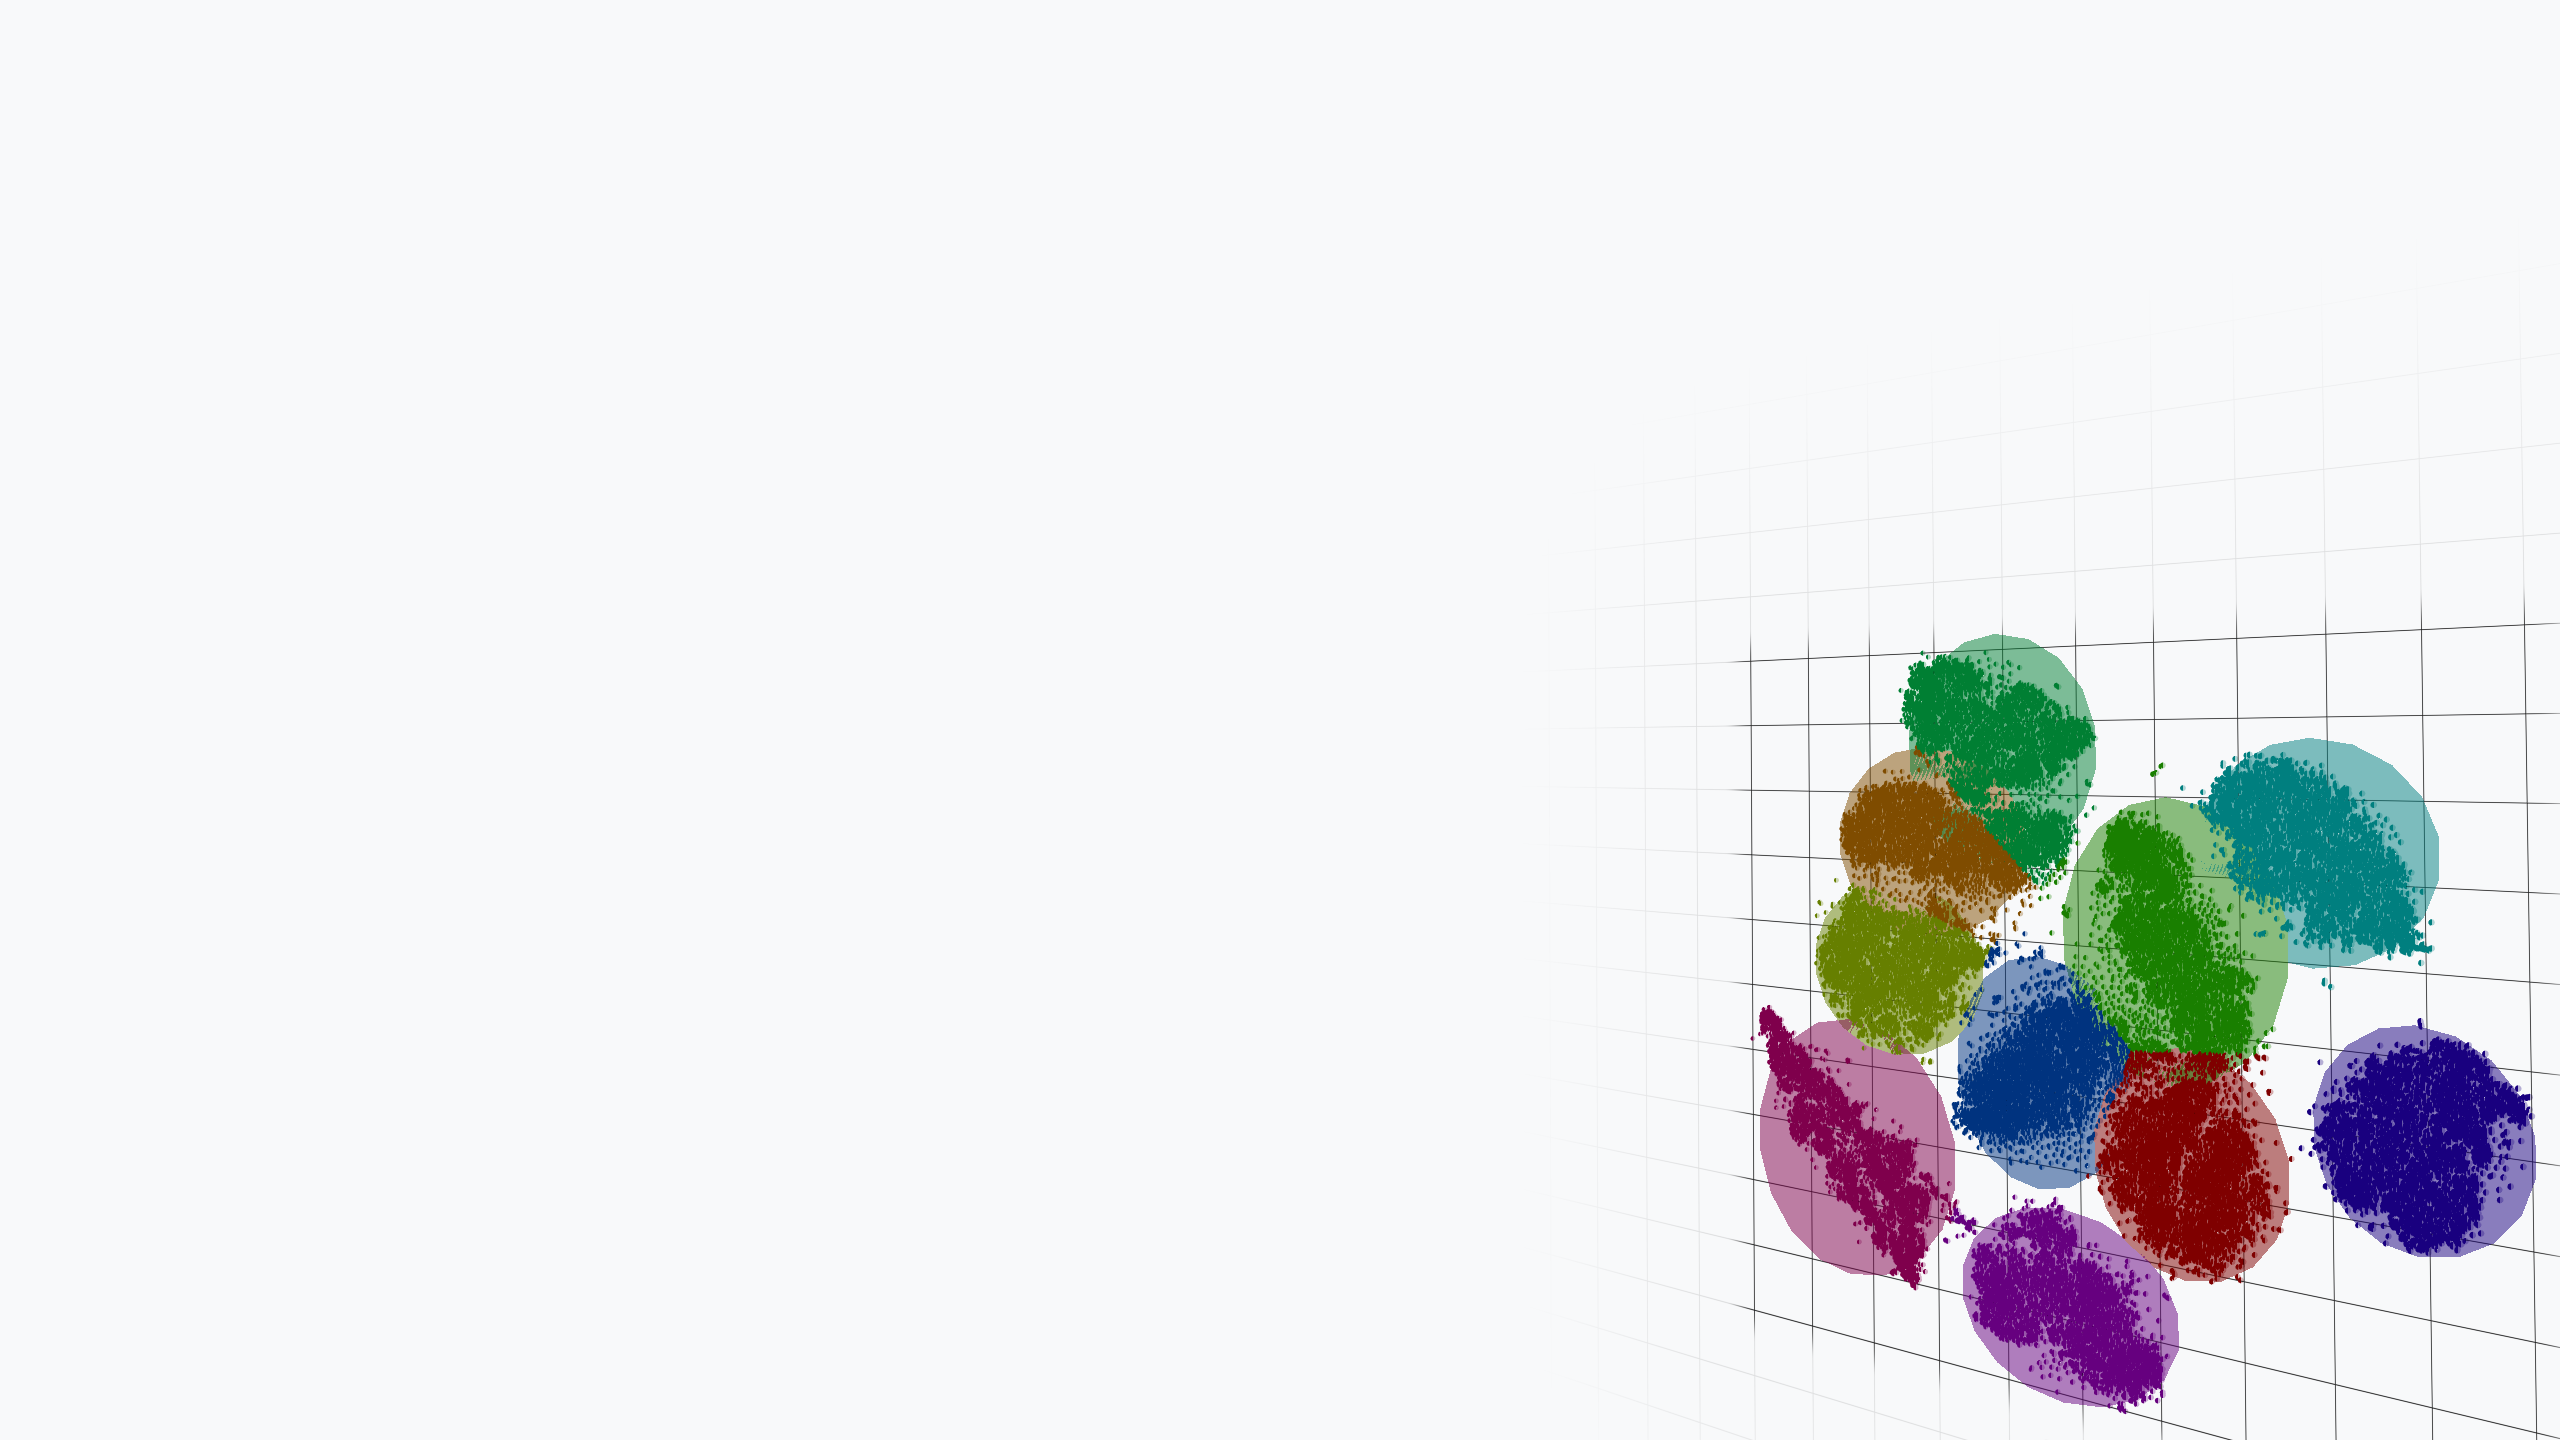
\includegraphics[height=\paperheight]{images/Download (19).png}}
\begin{frame}[plain]
	\titlepage
\end{frame} 
}

\begin{frame}[t]{Visualizing Huge Datasets}
	\bigskip
	\huge\textbf{Huge Datasets}

	\large\bigskip
	Increasingly digital world results in more and more data, \\overwhelming human comprehension

	\pause
	\bigskip
	Example dataset: Hathi Trust library catalog

	9 columns, ~5M rows, >600 MB .tsv
	\only<2->{\footnote{
		Data source: \href
			{http://creatingdata.us/data/scatter/hathi/tiles/}
			{creatingdata.us/data/scatter/hathi/tiles/}
	}}
\end{frame}

\begin{frame}[t]{Visualizing Huge Datasets}
	\bigskip
	\huge\textbf{First Approach: Use Excel}
	
	\pause
	\large\bigskip
	
\includegraphics[width=0.8\linewidth]{images/excelerror.png}

	\vspace*{-1.2cm}\hspace*{0.4\linewidth}
	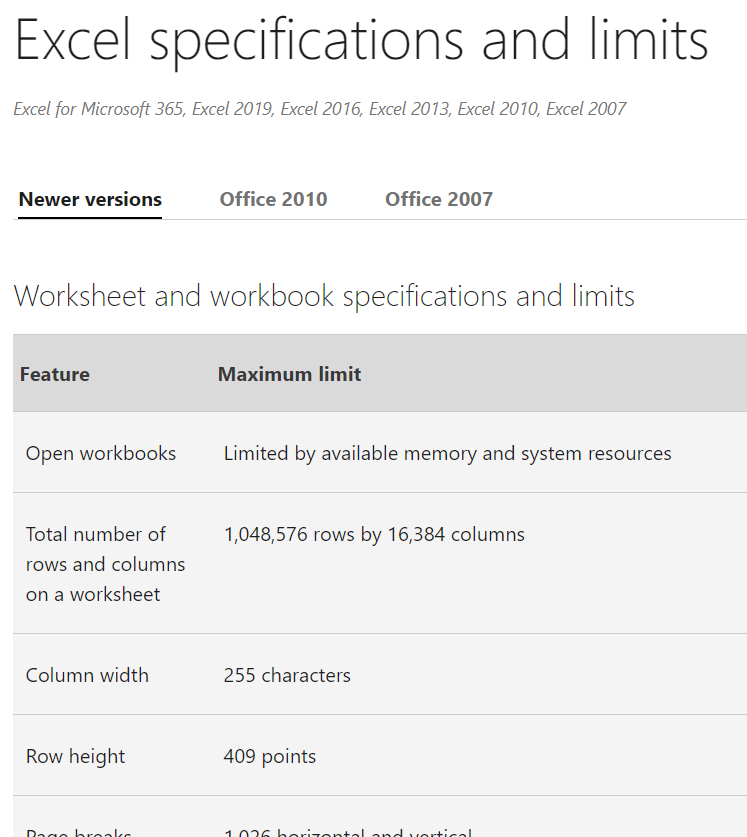
\includegraphics[trim=0 125 0 150, clip,width=0.6\linewidth]{images/excelspec.png}
	
	\vspace*{-2\baselineskip}
	5M rows is {\color{red}too much data} \\for Excel to visualize
\end{frame}

\begin{frame}[t]{Visualizing Huge Datasets}
	\bigskip
	\huge\textbf{Second Approach: \\Implement Viewer for a Specific Dataset}

	\large\bigskip
	Colin Eberhardt: \\\enquote{Rendering One Million Datapoints\\with D3 and WebGL}
	\footnote{
		Blog article: \href
			{https://blog.scottlogic.com/2020/05/01/rendering-one-million-points-with-d3.html}
			{blog.scottlogic.com/2020/05/01/rendering-one-million-points-with-d3.html}
		}%
	\textsuperscript{,}%
	\footnote{
		Demo: \href
			{https://colineberhardt.github.io/d3fc-webgl-hathi-explorer/}
			{colineberhardt.github.io/d3fc-webgl-hathi-explorer/}
	}

	\vspace*{-3\baselineskip}\hspace*{0.42\linewidth}
	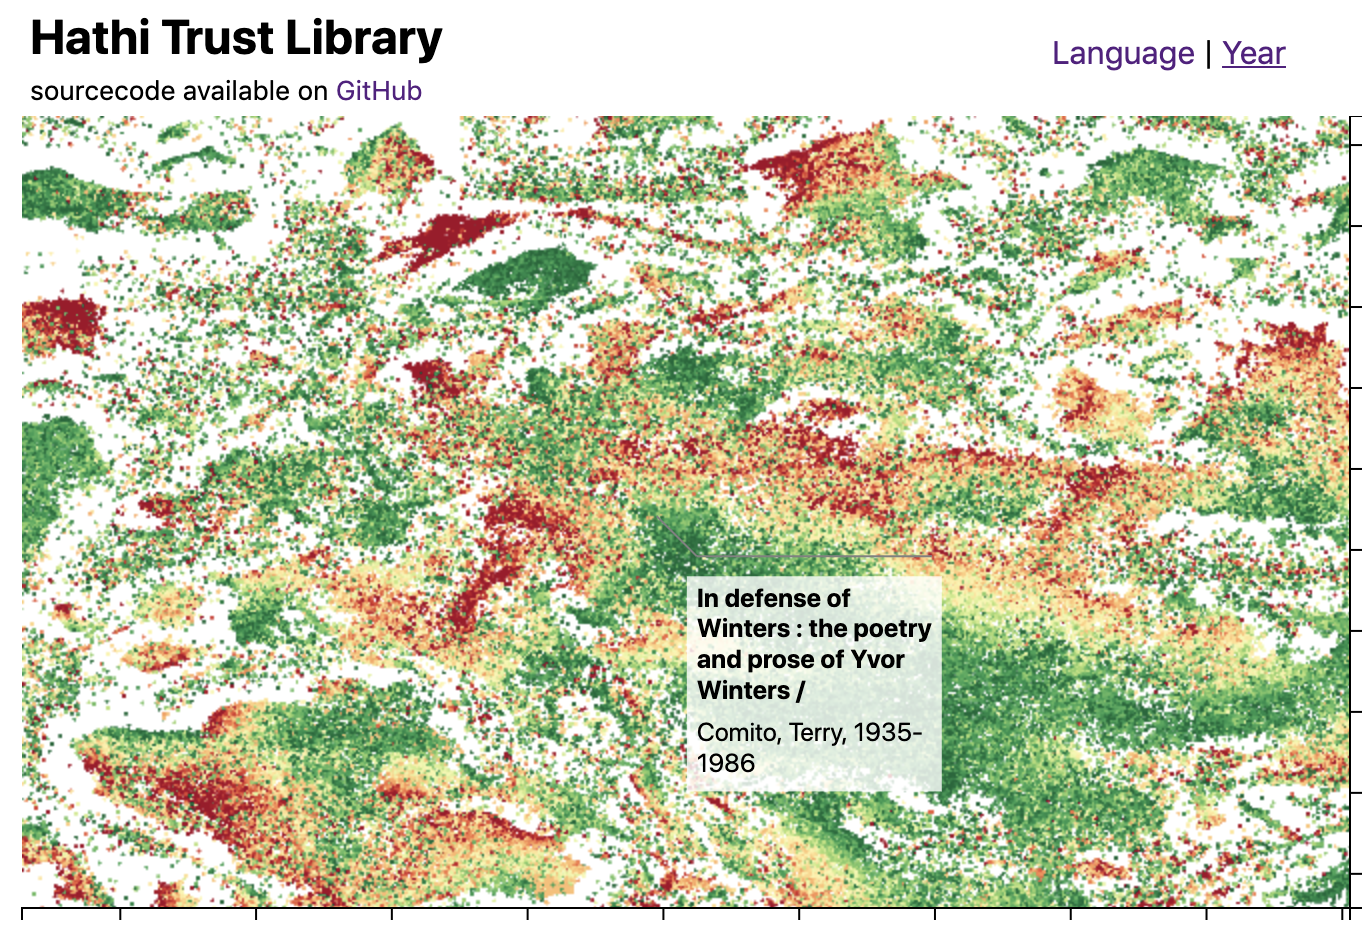
\includegraphics[trim=0 50 20 130,clip,width=0.58\linewidth]{images/hathi-library-visualisation.png}
	
	\pause
	\vspace*{-2\baselineskip}
	Works well, but optimized \\for {\color{red}specific} dataset 
\end{frame}

\begin{frame}[t]{Visualizing Huge Datasets}
	\bigskip
	\huge\textbf{Viewer Requirements}
	
	\large\bigskip
	\begin{description}[Dataset agnostic]
		\setlength{\itemsep}{5pt}
		\item[Huge datasets] Support datasets containing millions of datapoints
		\item[Dataset agnostic] Allow arbitrary mapping of columns to visual variables
		\item[Ease of access] Web-based implementation for cross-platform support \\without installation
	\end{description}
\end{frame}

\begin{frame}[t]{Demo}
	\bigskip
	\centering
	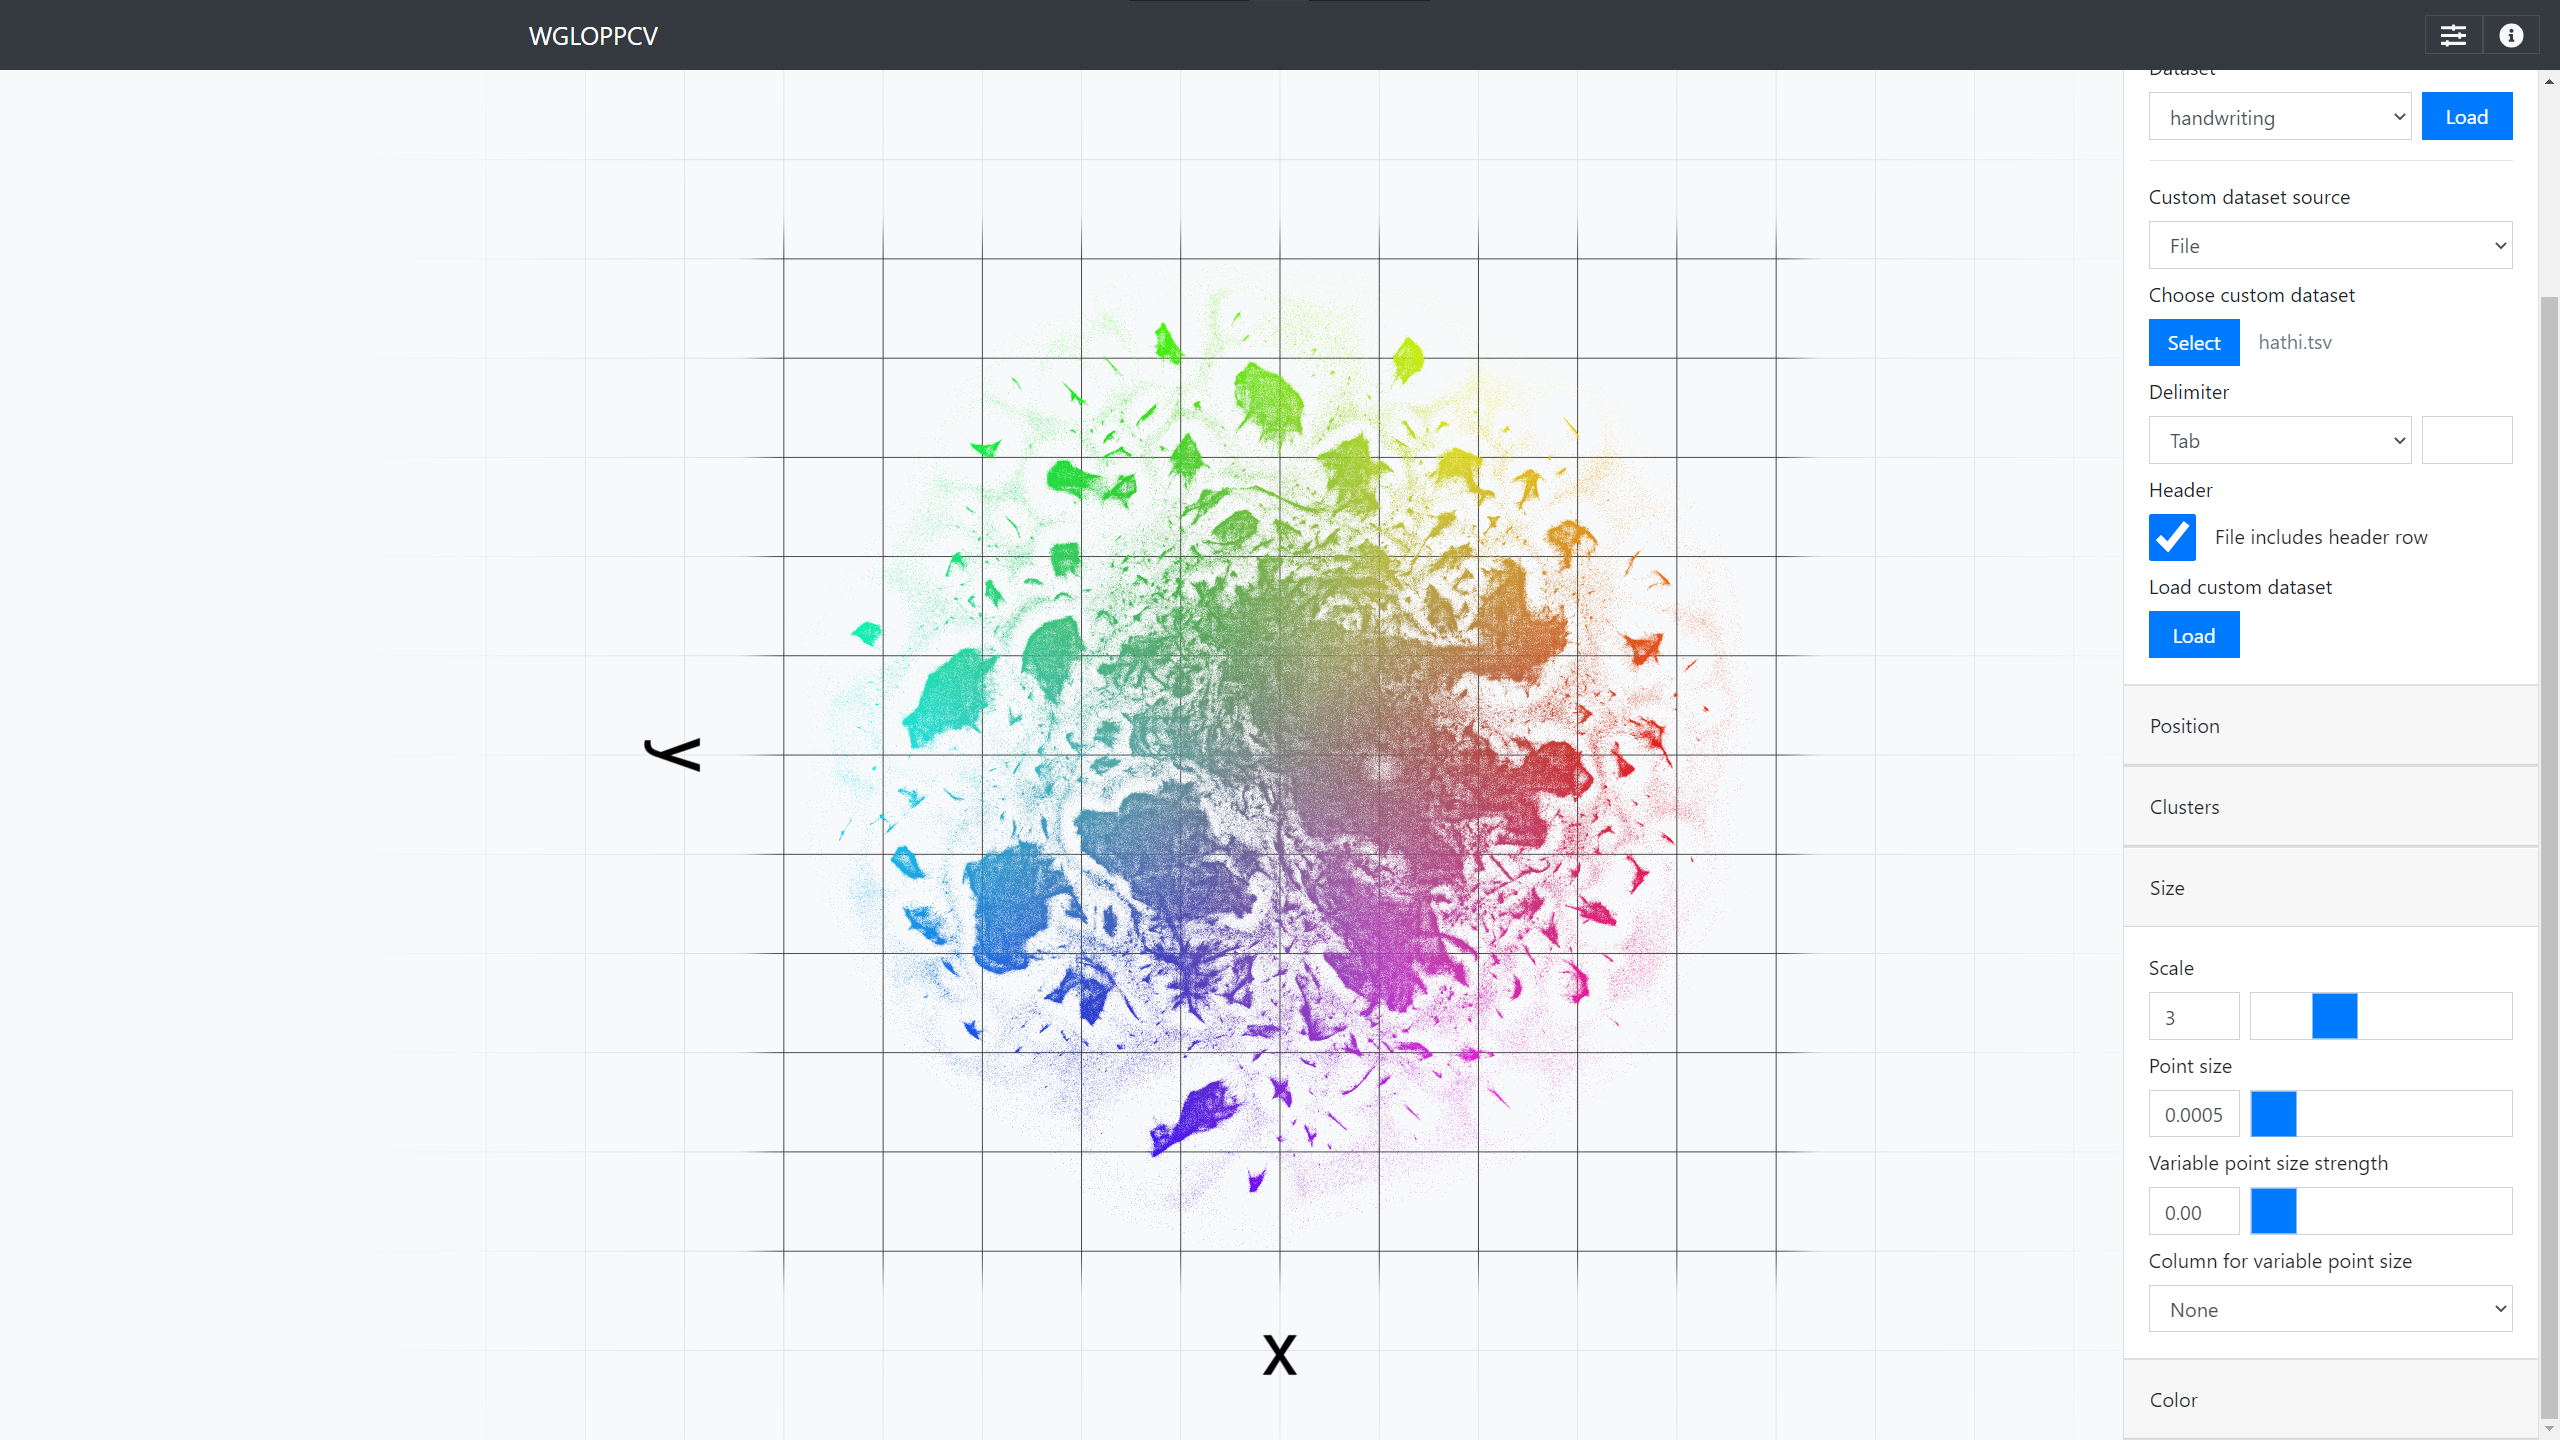
\includegraphics[trim=250 20 20 100,clip,width=0.75\linewidth]{images/hathi-tm-2.png}
\end{frame}

\begin{frame}[t]{Approach}
	\bigskip
	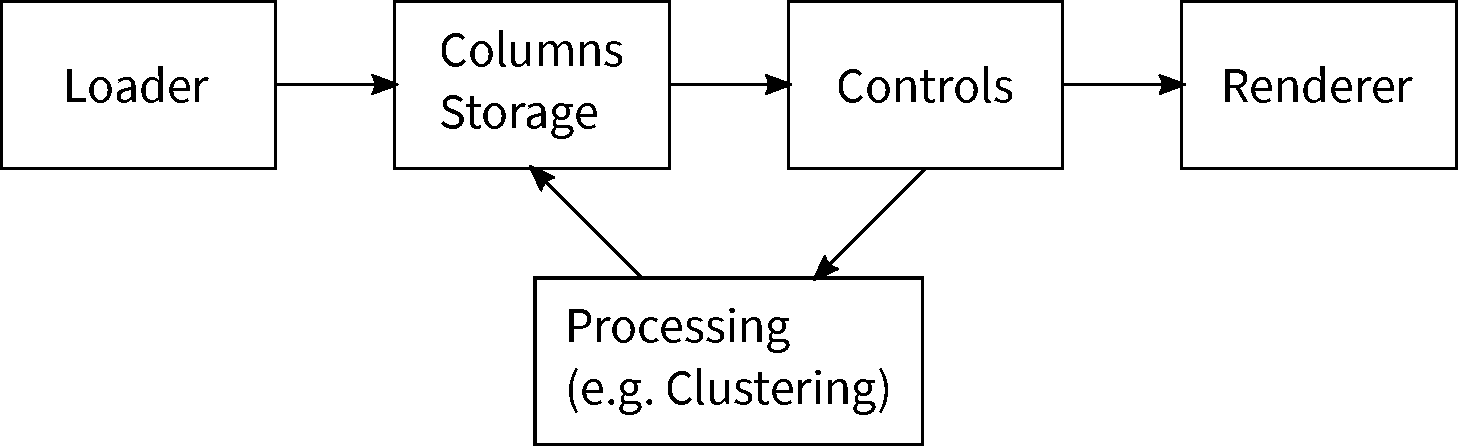
\includegraphics[width=0.7\linewidth]{images/flow.pdf}
	
	\bigskip
	\large
	Central storage of columns
	\begin{itemize}
		\item fed by modular loader (.csv, .tsv, ...)
		\item provides columns to be mapped to visual variables
		\item columns can also be used for processing steps
	\end{itemize}
\end{frame}

\begin{frame}[t]{Approach}
	\bigskip
	\large
	When configuring an output, only compatible columns are offered for selection
	\bigskip
	\begin{columns}[onlytextwidth]
		\begin{column}{0.5\textwidth}
			Visual variables:
			\begin{itemize}
				\item {\color<2>{blue}\{name: "x-coord", type: "number"\}}
				\item \{name: "y-coord", type: "number"\}
				\item \{name: "z-coord", type: "number"\}
				\item \{name: "size", type: "number"\}
				\item \{name: "color", type: "color"\}
			\end{itemize}
		\end{column}
		\begin{column}{0.5\textwidth}
			Available columns:
			\begin{itemize}
				\item {\color<2>{blue}\{name: "year", type: "number"\}}
				\item \{name: "country", type: "text"\}
				\item {\color<2>{blue}\{name: "ranking", type: "number"\}}
				\item {\color<2>{blue}\{name: "score", type: "number"\}}
				\item \{name: "jersey", type: "color"\}
			\end{itemize}
		\end{column}
	\end{columns}
\end{frame}

\begin{frame}[t]{Implementation}
	\bigskip
	\huge\textbf{Technology Stack}
	
	\large\bigskip
	\begin{columns}[onlytextwidth]
		\begin{column}[b]{0.33\textwidth}
			
\includegraphics[width=0.8\linewidth]{images/WebGL_Logo.pdf}
			
			\bigskip
			Rendering API: \\WebGL 2
		\end{column}
		\begin{column}[b]{0.33\textwidth}
			
\includegraphics[width=0.9\linewidth]{images/webgl-operate-logo.pdf}
			
			\bigskip
			Framework: \\webgl-operate
		\end{column}
		\begin{column}[b]{0.33\textwidth}
			
\includegraphics[width=0.6\linewidth]{images/ts-logo-512.pdf}
			
			\bigskip
			Language: \\TypeScript
		\end{column}
	\end{columns}
\end{frame}

\begin{frame}[t]{Implementation}
	\bigskip
	\huge\textbf{Optimized data handling}
	
	\large\bigskip
	Data is loaded and processed using Web Workers
	\begin{itemize}
		\item allows for parallel computing
		\item keep UI interactive by offloading work from main thread
	\end{itemize}

	\bigskip
	Web Workers are separate JS runtimes
	\begin{itemize}
		\item data has to be copied between workers
		\item solution: SharedArrayBuffers map the same memory location to multiple runtimes, improving speed and memory consumption
	\end{itemize}
\end{frame}

\begin{frame}[t]{Implementation}
	\bigskip
	\huge\textbf{Rendering Approach}
	
	\large\bigskip
	Rendering of millions of datapoints
	\begin{itemize}
		\item instanced rendering of a quad
		\footnote{\href{https://developer.mozilla.org/en-US/docs/Web/API/WebGL2RenderingContext/drawArraysInstanced}{developer.mozilla.org/en-US/docs/Web/API/WebGL2RenderingContext/drawArraysInstanced}}
		\item mapped columns are passed as per-instance attributes
	\end{itemize}
	
	\bigskip
	Separation of rendering into passes
	\begin{itemize}
		\item points, clusters, grid, labels are rendered by separate classes
		\item modularity allows for easy adjustments and extension
	\end{itemize}
\end{frame}

\begin{frame}[t]{Implementation}
	\bigskip
	\huge\textbf{Performance Measurements}
	
	\large\bigskip
	\begin{table}[]
		\begin{tabularx}{0.9\linewidth}{X|rrrrr}
			\toprule
			\textbf{Test System} & \multicolumn{5}{c}{\textbf{Number of Points}} \\
			in 1920$\times$1080px &\ $1\times10^6$ &\ $5\times10^6$ &\ $1\times10^7$ &\ $5\times10^7$ &\ $1\times10^8$ \\
			\midrule
			Intel UHD 630   &  26.8 &  18.6 &  10.8 &   2.6 &   1.4 \\
			Nvidia GTX 1650 & 196.6 &  65.2 &  38.0 &   8.9 &   4.6 \\
			Nvidia GTX 1080 & 474.6 & 154.3 &  81.2 &  17.6 &   9.0 \\
			\bottomrule
		\end{tabularx}
		\caption{Frames per second for different amounts of data measured on a low, mid, and high end GPU in Chrome 84.}
	\end{table}
\end{frame}

{
\usebackgroundtemplate{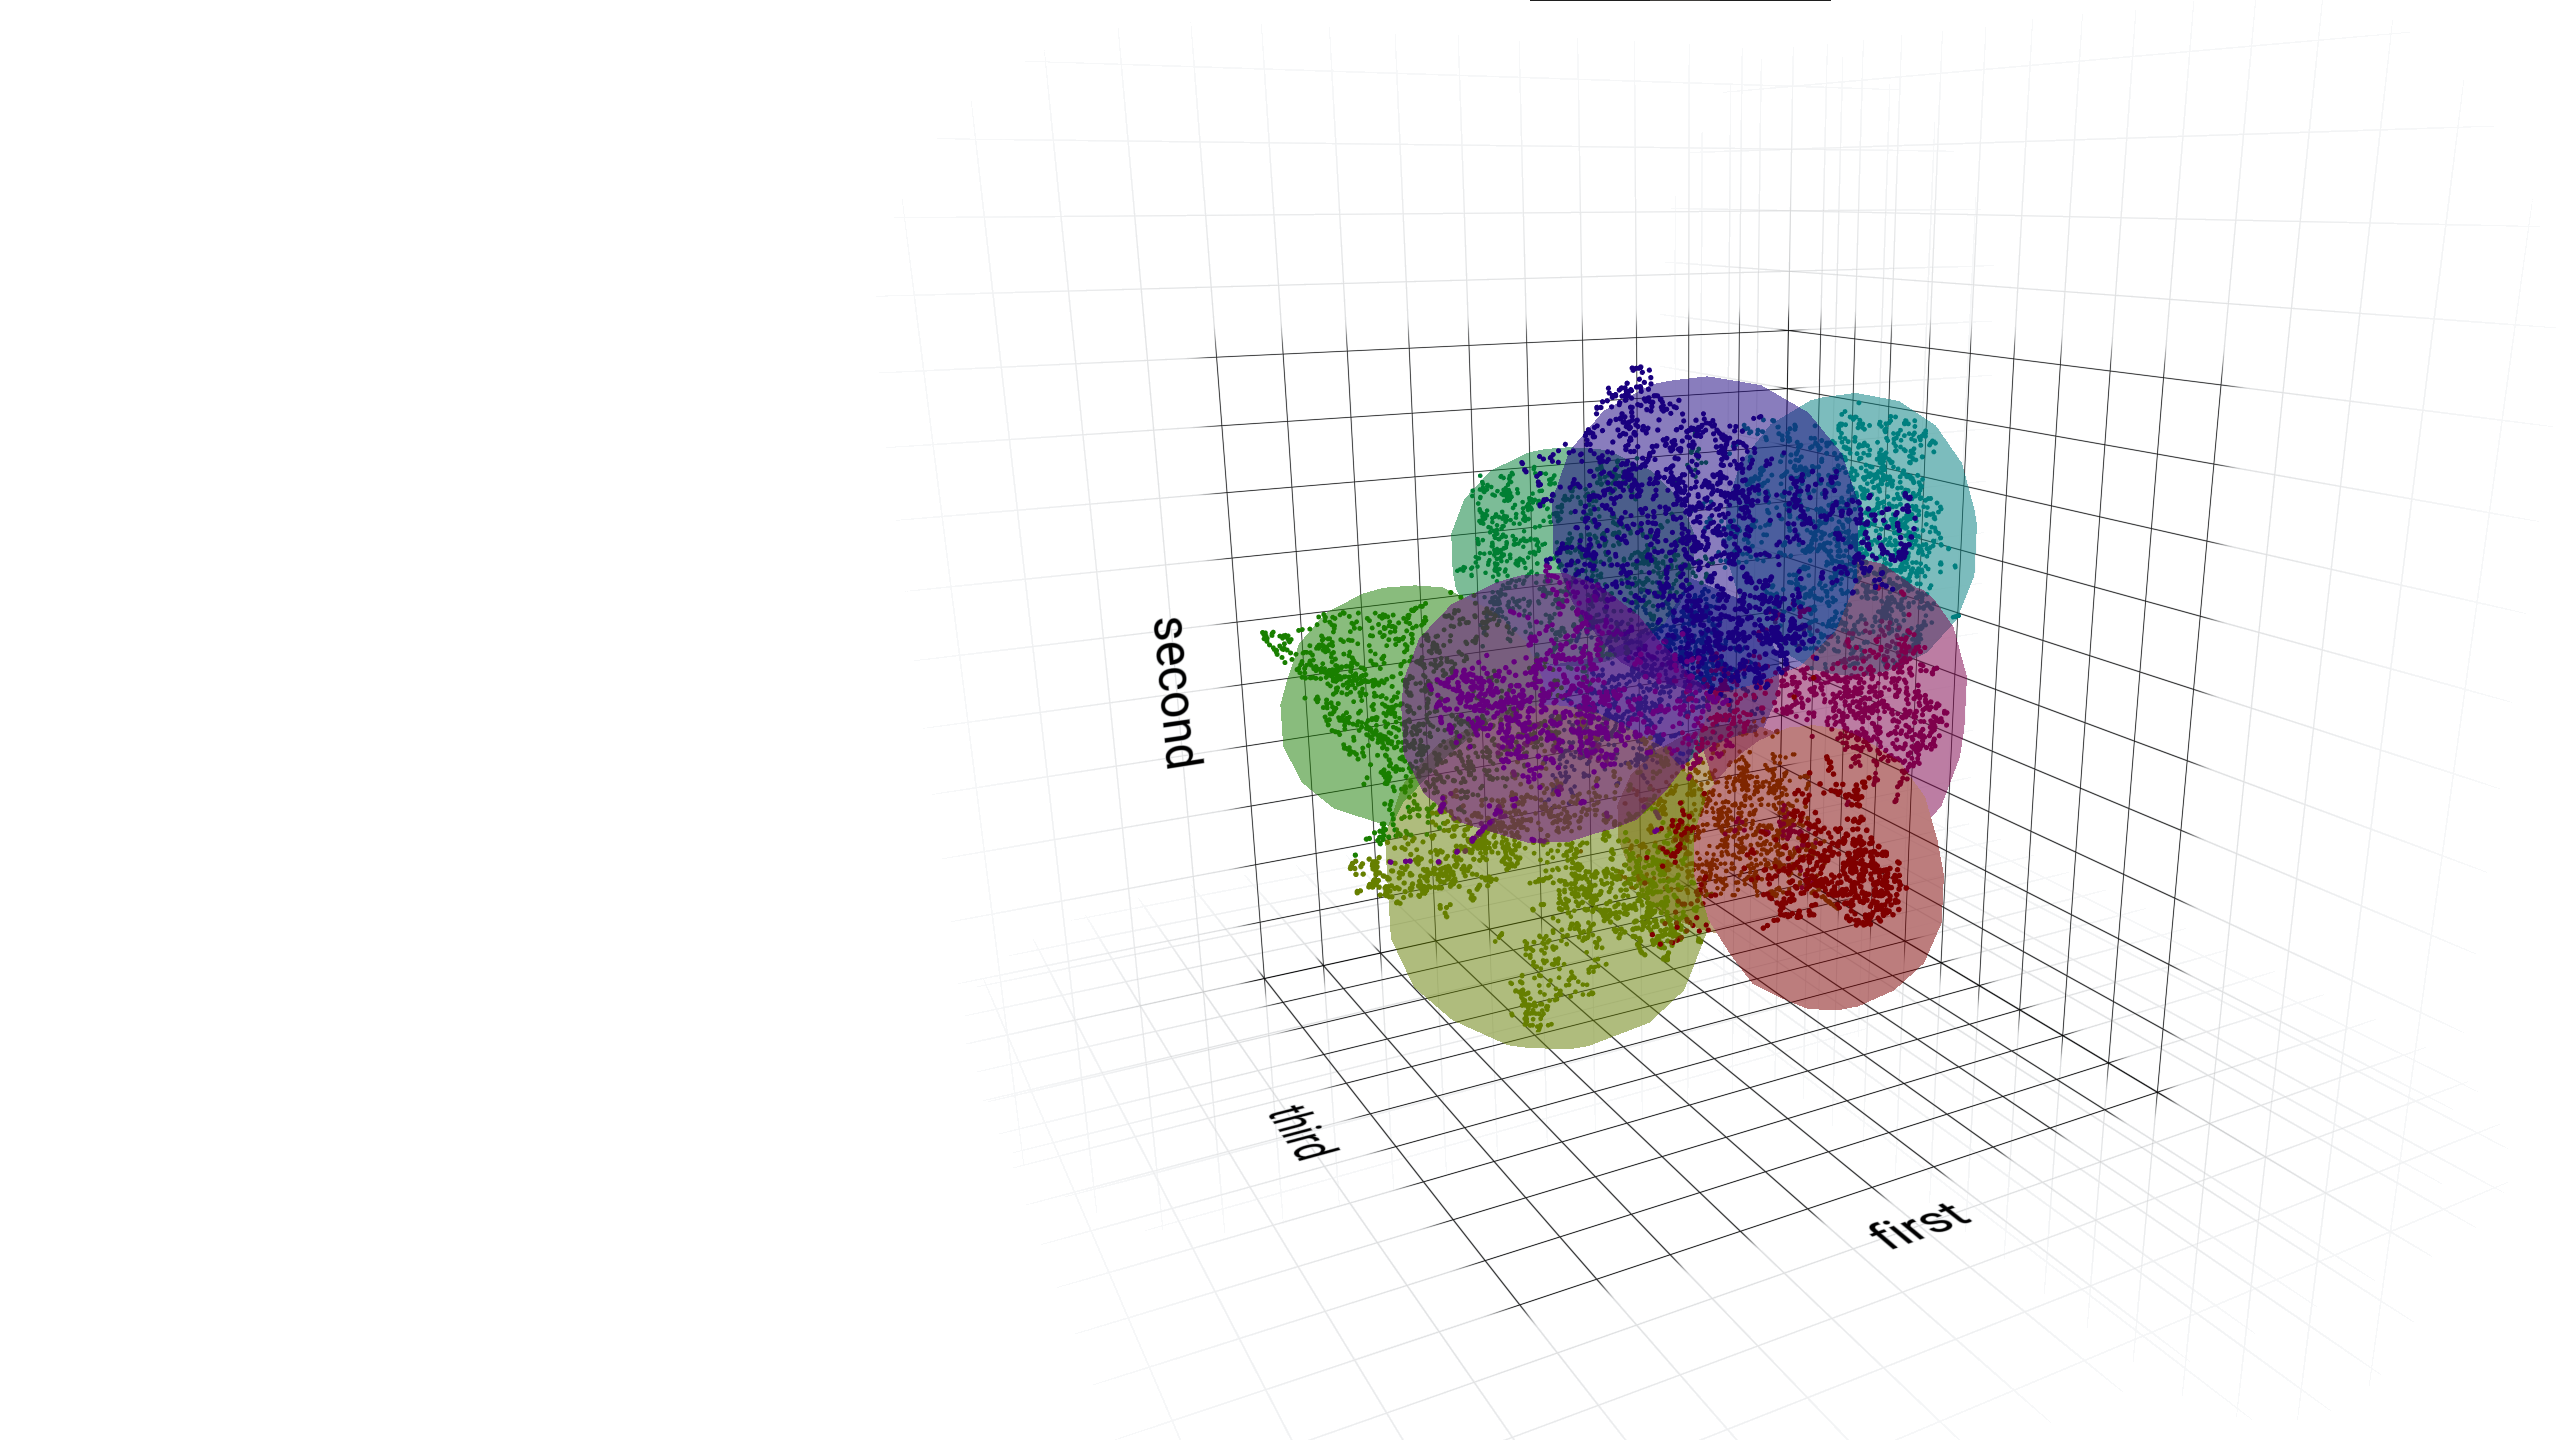
\includegraphics[height=\paperheight]{images/Screenshot 2020-10-29 172015.png}}
\begin{frame}[plain]
	\normalsize
	A Framework for Interactive Exploration of Clusters in Massive Data Using 3D Scatter Plots and WebGL
	
	\bigskip
	Wagner, Limberger, Scheibel, Trapp, D{\"o}llner
	
	\bigskip
	Contact: \href{mailto:lukas.wagner@hpi.de}{lukas.wagner@hpi.de}
	
	\bigskip
	Hasso Plattner Institute, \\University of Potsdam

	\vspace{3.5cm}
	\large
	Try it out: \href{https://varg.dev/web3d2020/}{varg.dev/web3d2020}
\end{frame} 
}

\end{document}
